{\bf 2026-10-21}\\

I have gotten the operator but each run produced about 150 GB of output, this is not feasible.

Fixes:
\begin{itemize}
    \item Stopped outputting rcond and cov maps, I can output these again later if I need them.
    \item Starting simulating `partial' maps that are blank outside of the region of interest.
    \item Started saving the maps as h5py files instead of fits files, this saves a lot of space as the h5py file only save `submaps' in which there are hits.
\end{itemize}

All of these things required reworking various codes to be able to read the new types of maps.

To date, most of my maps have been built with an nside of $2^{13}$, this is around the limit of what I can easily do with the sim sky map code. Perhaps with partial maps I could increase this, but ideally to get high resolution maps of a point source I would need higher nside.

\begin{figure}
    \centering
    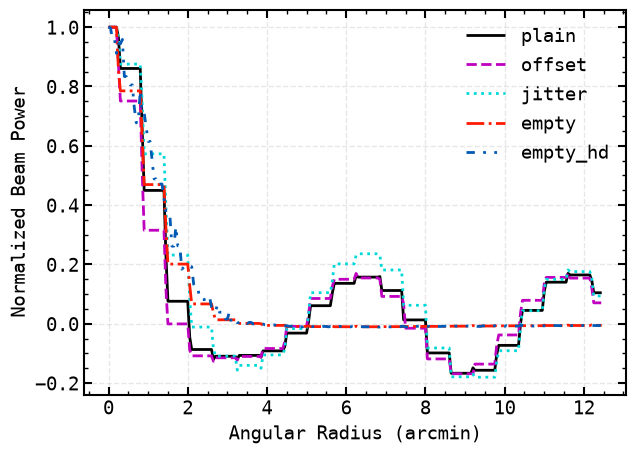
\includegraphics[width=0.5\textwidth]{Updates/figures/lowres_radprofiles.png}
    \caption{Caption for the figure}
\end{figure}

I removed the \verb+--scan_map+ arguments so that the sim would assume an empty sky, but I left the \verb+sim_sso+ arguments. With this, I then boosted the nside to $2^{15}$ to try and get a high res point source map. I ran this with both no jitter, and 30 arcsec jitter (might actually be 1 arcmin I can't remember).

\begin{figure}
    \centering
    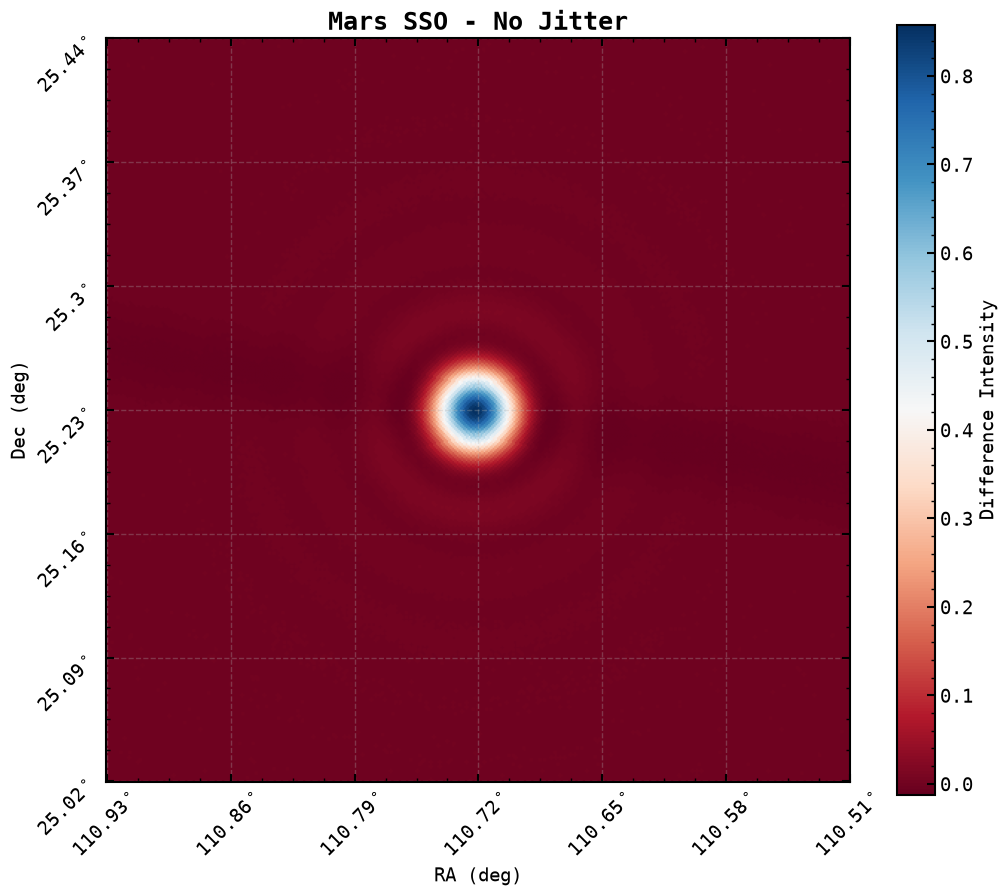
\includegraphics[width=0.75\textwidth]{Updates/figures/HD_mars_sso.png}
    \caption{Caption for the figure}
\end{figure}
\begin{figure}
    \centering
    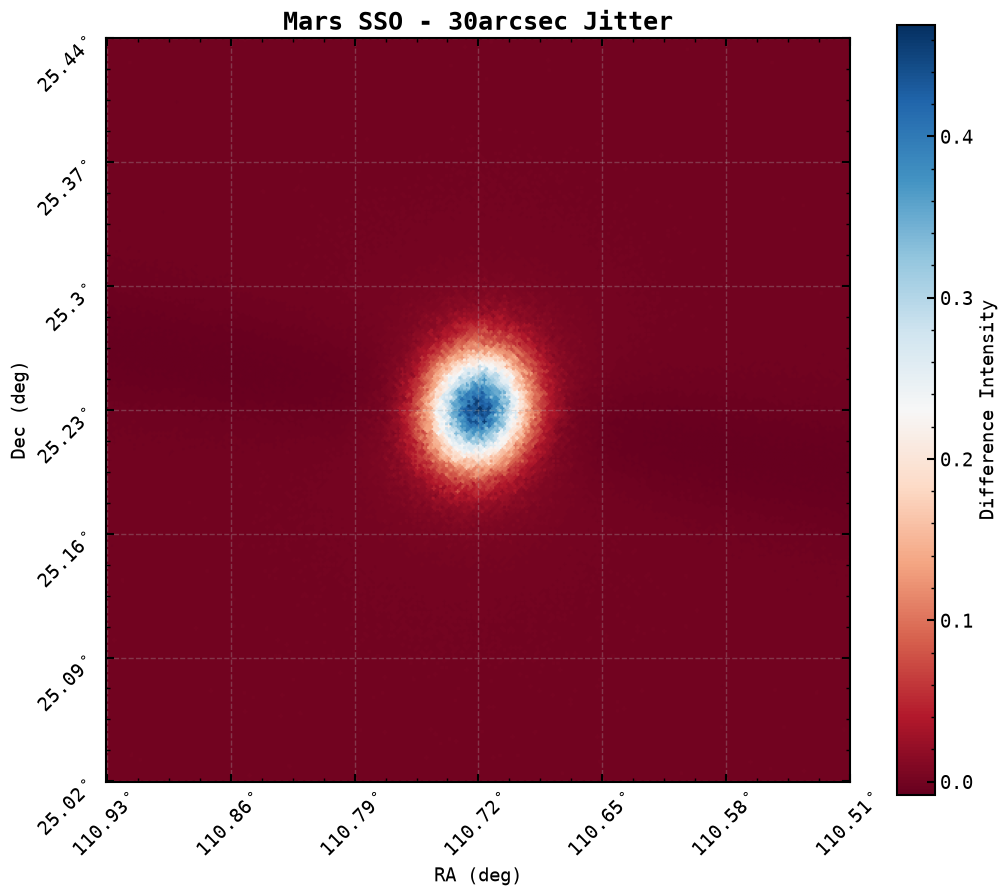
\includegraphics[width=0.75\textwidth]{Updates/figures/HD_mars_jitter_sso.png}
    \caption{Caption for the figure}
\end{figure}


\begin{figure}
    \centering
    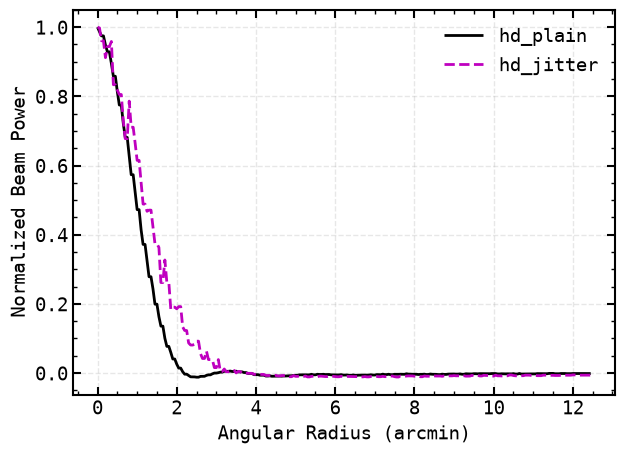
\includegraphics[width=0.5\textwidth]{Updates/figures/hd_radprofiles.png}
    \caption{Caption for the figure}
\end{figure}